% ЕМТ 2025, VI клас — точен LaTeX препис от официалните файлове в Klasirane.com.
% Условия: https://klasirane.com/api/competitions/EMT/All/2025/6%20%D0%BA%D0%BB/probs
% SHA-256 (условия): 150140d83aaf7ab2e18d8f499042cbf8c6afaf7b66eeebae091ee0dc2523b78d
% Решения: https://klasirane.com/api/competitions/EMT/All/2025/6%20%D0%BA%D0%BB/sol
% SHA-256 (решения): 74ed321555cf615d981fcdaa561f24e0f45c00fcb28f431812b1750dc19637db
% Точковите оценки, правописът и непълнотите са запазени от източника.

Задача 6.1. По маршрута на велопоход има 9 пункта за вода – първият е на старта, а деветият е на финала. Пунктовете са на равни разстояния един от друг.

Георги стартирал в 8:00 часа и когато изминал $\dfrac{1}{3}$ от маршрута, пресметнал, че му остават още 3 km до следващия пункт за вода.

а) Колко километра е дължината на маршрута?

б) Георги и Иван пристигнали на финала в 12:00 часа. Ако скоростта на Георги е била с 20% по-малка от скоростта на Иван, намерете в колко часа е стартирал Иван.

Решение. а) Пунктовете за вода разделят маршрута на 8 равни части. Тъй като

$$\dfrac{2}{8}<\dfrac{1}{3}<\dfrac{3}{8},$$

в момента, в който Георги е изминал $\dfrac{1}{3}$ от маршрута, до следващия пункт му остава

$$\dfrac{3}{8}-\dfrac{1}{3}=\dfrac{1}{24}$$

от маршрута, което по условие е 3 km. Следователно дължината на маршрута е $24\cdot3=72$ km.

(3 точки)

б) Ако скоростта на Иван е $x$ km/h, то скоростта на Георги е $80\%x$. Тъй като Георги е изминал пътя за 4 часа, неговата скорост е била $72:4=18$ km/h. Получаваме

$$80\%x=18,$$

откъдето $x=22,5$ km/h.

(2 точки)

Иван е изминал маршрута за $72:22,5=3,2$ h, т.е. за 3 h 12 min. Щом е финиширал в 12:00, той е стартирал в 8:48.

(1 точка)

Задача 6.2. В клетките на таблица с 2 реда и 60 стълба последователно се записват числа по следния начин:

• в двете клетки на първия стълб се записва числото 5;

• на първия ред във всяка клетка след първата се записва число, равно на $(x-1):(x+1)$, където $x$ е числото в предишната клетка в първия ред;

• на втория ред във всяка клетка след първата се записва число, равно на $(x-1):(x+2)$, където $x$ е числото в предишната клетка във втория ред.

В колко колони на таблицата са записани две равни числа?

Решение. Второто число на първия ред е

$$(5-1):(5+1)=\dfrac{2}{3},$$

третото е

$$\left(\dfrac{2}{3}-1\right):\left(\dfrac{2}{3}+1\right)=-\dfrac{1}{5},$$

четвъртото е

$$\left(-\dfrac{1}{5}-1\right):\left(-\dfrac{1}{5}+1\right)=-\dfrac{3}{2},$$

петото е

$$\left(-\dfrac{3}{2}-1\right):\left(-\dfrac{3}{2}+1\right)=5.$$

Това означава, че на първия ред периодично се повтарят числата $5$, $\dfrac{2}{3}$, $-\dfrac{1}{5}$, $-\dfrac{3}{2}$. (2 точки)

На втория ред второто число е

$$(5-1):(5+2)=\dfrac{4}{7},$$

третото е

$$\left(\dfrac{4}{7}-1\right):\left(\dfrac{4}{7}+2\right)=-\dfrac{1}{6},$$

четвъртото е

$$\left(-\dfrac{1}{6}-1\right):\left(-\dfrac{1}{6}+2\right)=-\dfrac{7}{11},$$

петото е

$$\left(-\dfrac{7}{11}-1\right):\left(-\dfrac{7}{11}+2\right)=-\dfrac{6}{5},$$

шестото е

$$\left(-\dfrac{6}{5}-1\right):\left(-\dfrac{6}{5}+2\right)=-\dfrac{11}{4},$$

седмото е

$$\left(-\dfrac{11}{4}-1\right):\left(-\dfrac{11}{4}+2\right)=5.$$

Следователно на втория ред периодично се повтарят числата $5$, $\dfrac{4}{7}$, $-\dfrac{1}{6}$, $-\dfrac{7}{11}$, $-\dfrac{6}{5}$, $-\dfrac{11}{4}$. (3 точки)

Колона с две равни числа може да се получи, само ако и в двете клетки на тази колона е записано числото 5. Тъй като $\operatorname{НОК}(4;6)=12$, колоните с равни числа са $60:12=5$.

(1 точка)

Задача 6.3. Даден е триъгълник $ABC$. Върху страната $AB$ са избрани точки $D$ и $E$ така, че $D$ е между $A$ и $E$, а върху страната $AC$ са избрани точки $P$, $M$ и $N$ в този ред, считано от върха $A$.

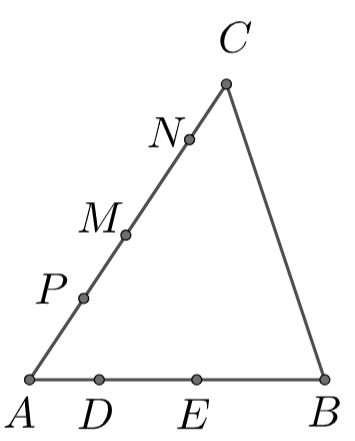
\includegraphics[max width=0.42\textwidth, alt={Триъгълник ABC с точки D и E върху AB и P, M и N върху AC}, center]{assets/6-3-triangle.png}

Дадените точки разделят страните на триъгълника, като:

$$AD=\dfrac{1}{a}\cdot AB,\quad DE=\dfrac{1}{b}\cdot AB,\quad EB=\dfrac{1}{c}\cdot AB,$$

$$AP=\dfrac{1}{p}\cdot AC,\quad PM=\dfrac{1}{m}\cdot PC,\quad MN=\dfrac{1}{n}\cdot MC,$$

където $a$, $b$, $c$, $n$, $m$, $p$ са едноцифрени естествени числа и

$$a<b<c<n<m<p.$$

а) Намерете числата $a$, $b$, $c$, $n$, $m$, $p$.

б) Разстоянията от точките $P$, $M$ и $N$ до правата $AB$ са равни съответно на $h_1$, $h_2$ и $h_3$, а разстоянията от точките $D$ и $E$ до правата $AC$ са равни съответно на $h_4$ и $h_5$. Ако

$$2(h_1+h_2+h_3)=h_4+h_5,$$

докажете, че триъгълникът $ABC$ е равнобедрен.

Решение. а) От $AD+DE+EB=AB$ следва, че

$$\dfrac{1}{a}+\dfrac{1}{b}+\dfrac{1}{c}=1.$$

Единствените различни едноцифрени числа, за които това равенство е изпълнено, са $a=2$, $b=3$, $c=6$. (Ясно е, че $a$ не може да е 1; най-голямото събираемо в сбора е $\dfrac{1}{a}$, следователно $\dfrac{1}{a}>\dfrac{1}{3}$, откъдето следва, че $a=2$. Тогава $\dfrac{1}{b}+\dfrac{1}{c}=\dfrac{1}{2}$ и тъй като $\dfrac{1}{b}>\dfrac{1}{c}$, получаваме $\dfrac{1}{b}>\dfrac{1}{4}$, следователно $b=3$, а $c=6$.)

Тъй като всички търсени числа са едноцифрени, подредени в нарастващ ред, то $n=7$, $m=8$, $p=9$.

(2 точки)

б) Нека с $h_b$ и $h_c$ означим височините в триъгълника $ABC$ към страните $AC$ и $AB$ съответно.

От $AP=\dfrac{1}{9}AC$ следва, че $S_{APB}=\dfrac{1}{9}S_{ABC}$, а тъй като тези триъгълници имат обща страна $AB$, получаваме, че $h_1=\dfrac{1}{9}h_c$.

От $PM=\dfrac{1}{8}\cdot PC=\dfrac{1}{8}\cdot\dfrac{8}{9}AC=\dfrac{1}{9}AC$ следва, че $AM=\dfrac{2}{9}AC$, откъдето $S_{AMB}=\dfrac{2}{9}S_{ABC}$, а тъй като тези триъгълници имат обща страна $AB$, получаваме, че $h_2=\dfrac{2}{9}h_c$.

По същия начин, от $MN=\dfrac{1}{7}\cdot MC=\dfrac{1}{7}\cdot\dfrac{7}{9}AC=\dfrac{1}{9}AC$ следва, че $AN=\dfrac{3}{9}AC$, откъдето $S_{ANB}=\dfrac{3}{9}S_{ABC}$, а тъй като тези триъгълници имат обща страна $AB$, получаваме, че $h_3=\dfrac{3}{9}h_c$.

Следователно

$$2(h_1+h_2+h_3)=2\cdot\dfrac{1+2+3}{9}h_c=\dfrac{4}{3}h_c.$$

(2 точки)

От $AD=\dfrac{1}{2}AB$ следва, че $S_{ADC}=\dfrac{1}{2}S_{ABC}$, а тъй като тези триъгълници имат обща страна $AC$, получаваме, че $h_4=\dfrac{1}{2}h_b$.

От $AE=\dfrac{5}{6}AB$ следва, че $S_{AEC}=\dfrac{5}{6}S_{ABC}$, а тъй като тези триъгълници имат обща страна $AC$, получаваме, че $h_5=\dfrac{5}{6}h_b$.

Следователно

$$h_4+h_5=\dfrac{1}{2}h_b+\dfrac{5}{6}h_b=\dfrac{4}{3}h_b.$$

(2 точки)

Като заместим в даденото равенство $2(h_1+h_2+h_3)=h_4+h_5$, получаваме, че $h_c=h_b$. Следователно $AB=AC$, т.е. триъгълникът $ABC$ е равнобедрен.

(1 точка)

Задача 6.4. Равностранен триъгълник със страна 45 cm е разделен на клетки с форма на равностранен триъгълник със страна 1 cm (виж фигура 1). В някои две клетки от триъгълника са поставени паяк и скакалец.

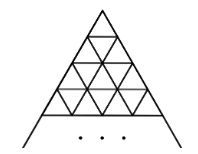
\includegraphics[max width=0.34\textwidth, alt={Фигура 1: начало на мрежата от единични равностранни триъгълници}, center]{assets/6-4-grid-fragment.png}

Паякът с един ход може да се премести във всяка клетка, която има обща страна или връх с тази, в която се намира (фигура 2). В никоя клетка той не стъпва повече от веднъж.

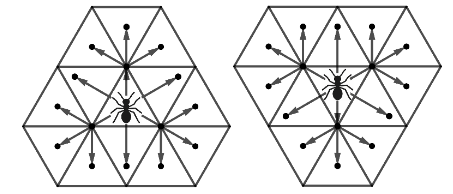
\includegraphics[max width=0.58\textwidth, alt={Фигура 2: възможните ходове на паяка от двата вида триъгълни клетки}, center]{assets/6-4-spider-moves.png}

Скакалецът за един ход прескача по три клетки в показаните посоки и скача в една от шестте клетки, посочени със стрелки на фигура 3. В никоя клетка той не стъпва повече от веднъж.

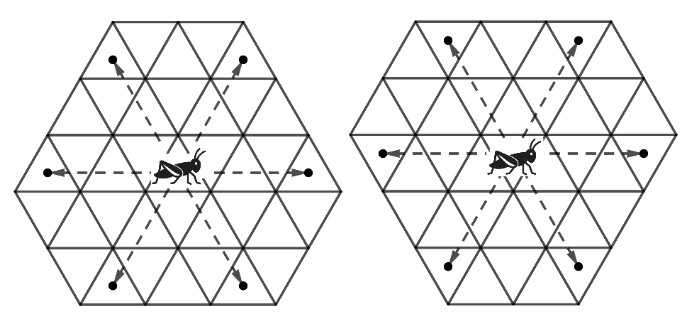
\includegraphics[max width=0.78\textwidth, alt={Фигура 3: шестте възможни посоки за скок на скакалеца}, center]{assets/6-4-grasshopper-moves.png}

Най-много колко клетки може да посети всяко насекомо?

Посочете (чрез пример) от коя клетка тръгва насекомото и как се движи, за да посети най-много клетки. Докажете, че не може да посети по-голям брой клетки.

Решение. Ако поставим паяка в клетка във връх на триъгълника, той може да обиколи всички клетки ред по ред.

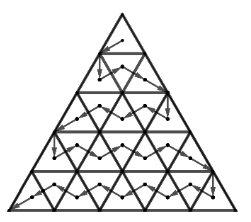
\includegraphics[max width=0.42\textwidth, alt={Маршрутът на паяка ред по ред}, center]{assets/6-4-spider-route.png}

На първия ред има 1 клетка, на втория 3, на третия 5 и т.н. На 45-ия ред има $45\cdot2-1=89$ клетки. Следователно общият брой клетки, които може да обходи паякът, е

$$1+3+5+\cdots+87+89=45\cdot90:2=2025.$$

(2 точки)

Нека поставим скакалеца в някоя от клетките, които се намират във връх на триъгълника. Оцветяваме тази клетка в черно и продължаваме да оцветяваме през ред, като оцветяваме първата и и всяка четвърта клетка по този ред. При това оцветяване, ако скакалецът тръгне от черна клетка, той винаги попада отново в черна.

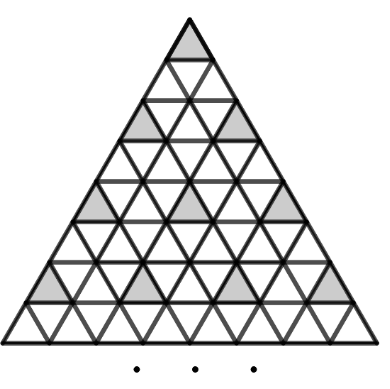
\includegraphics[max width=0.42\textwidth, alt={Черните клетки, до които може да скача скакалецът}, center]{assets/6-4-black-cells.png}

Скакалецът може да обиколи всички черни клетки, като мине последователно по нечетните редове, както е показано на схемата.

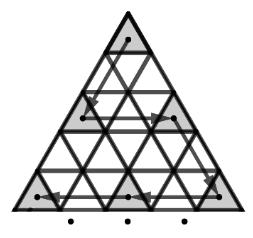
\includegraphics[max width=0.38\textwidth, alt={Маршрутът на скакалеца по нечетните редове}, center]{assets/6-4-grasshopper-route.png}

Общият брой на оцветените клетки е

$$1+2+\cdots+23=\dfrac{23\cdot24}{2}=276.$$

(3 точки)

За да се убедим, че по-дълъг маршрут е невъзможен, ще оцветим клетките в осем цвята. На чертежа във всяка клетка е записан номерът на нейния цвят; на нечетните редове се редуват цветовете 1, 5, 6, 7, а на четните редове се редуват цветовете 2, 4, 3, 8. При това оцветяване скакалецът може да посещава клетки само от един и същ цвят.

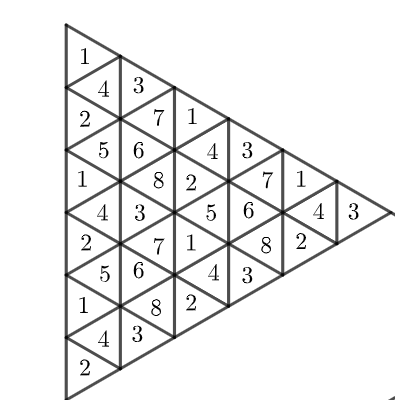
\includegraphics[max width=0.58\textwidth, alt={Оцветяване на клетките с осем цвята, означени с числата от 1 до 8}, center]{assets/6-4-eight-colors.png}

Клетките от всеки от цветовете 2, 3, 4, 5, 6 и 7, са $1+2+\cdots+22=\dfrac{22\cdot23}{2}=253$, а клетките от цвят 8 са $1+2+\cdots+21=\dfrac{21\cdot22}{2}=231$.

(2 точки)
